\documentclass[11pt]{article}

\usepackage[margin=2.4cm]{geometry}
\usepackage[utf8]{inputenc}
\usepackage[T1]{fontenc}
\usepackage{lmodern}
\usepackage{amsmath}
\usepackage{amssymb}
\usepackage{graphicx}
\usepackage{booktabs}
\usepackage{longtable}
\usepackage{array}
\usepackage{listings}
\usepackage{xcolor}
\usepackage{hyperref}
\usepackage{caption}
\usepackage{parskip}
\usepackage{fancyhdr}

\hypersetup{colorlinks=true, linkcolor=blue, citecolor=blue, urlcolor=blue}

\newcolumntype{L}[1]{>{\raggedright\arraybackslash}p{#1}}

\lstdefinestyle{pseudo}{
  basicstyle=\ttfamily\footnotesize,
  breaklines=true,
  columns=fullflexible,
  frame=single,
  numbers=left,
  numberstyle=\tiny\color{gray},
  keywordstyle=\bfseries,
  commentstyle=\color{teal},
  keywords={if,else,while,for,to,return,signal,and,or,not,mod},
  morecomment=[l]{//},
}

\lstdefinestyle{code}{
  basicstyle=\ttfamily\footnotesize,
  breaklines=true,
  columns=fullflexible,
  frame=single,
  numbers=left,
  numberstyle=\tiny\color{gray},
  keywordstyle=\bfseries\color{blue!60!black},
  commentstyle=\color{teal},
  stringstyle=\color{orange!70!black},
  language=Python,
}

\setlength{\headheight}{14pt}
\pagestyle{fancy}
\fancyhf{}
\fancyhead[L]{SOEN 6011 -- F2 tan(x) -- Deliverable 1}
\fancyhead[R]{\thepage}

\title{\textbf{A User-Centred, From-Scratch Scientific Calculator\\ for the Tangent Function $\tan(x)$}\\[0.3cm]
\large Deliverable 1: Persona, Requirements, Algorithms, CLI Prototype}
\author{Risat Ahmed \\ Student ID: 40294116 \\ SOEN 6011 -- Software Engineering Processes, Section CC \\ Concordia University -- Summer 2026}
\date{July 15, 2026}

\begin{document}

\maketitle
\thispagestyle{empty}
\newpage

\tableofcontents
\newpage

\section{Introduction}

This report documents Deliverable 1 (D1) of a medium-sized scientific software engineering project: a user-centred, eventually from-scratch, scientific calculator implementing the real tangent function
\[
\tan(x) = \frac{\sin(x)}{\cos(x)}, \qquad x \in \mathbb{R},
\]
with $x$ expressed in radians. The tangent function has period $\pi$, is odd ($\tan(-x) = -\tan(x)$), has range equal to all real numbers, and is undefined at the poles $x = \pi/2 + k\pi$ ($k \in \mathbb{Z}$), where $\cos(x) = 0$. D1 covers four problems, each informed by the previous one: a user persona (Problem 1), requirements expressed per ISO/IEC/IEEE~29148 (Problem 2), two language-independent algorithms in pseudocode (Problem 3), and an algorithm selection plus a runnable Python command-line prototype (Problem 4).

Per constraint C-03, every problem below used a public generative AI (GAI) tool with a CASTROFF-structured prompt (Task, Restrictions, Output Format, Audience); the exact prompts, output evaluation, and verification method for each problem are given in their respective subsections and summarized in Appendix~\ref{sec:gai-log}.

\textbf{Working assumptions (Step 0, pending final professor confirmation --- see Section~\ref{sec:decisions}):} angle unit is radians; the supported argument range is $|x| \le 10^4$ radians; inputs within a small tolerance of a pole are rejected rather than computed.

\section{Problem 1 --- Persona}

\subsection{GAI tool and prompt}
\textbf{Tool:} Claude Code (Claude, Anthropic, Sonnet 5 model), accessed 2026-07-15. \textbf{Prompt type:} Generative + decision-support (persona synthesis informed by a template-selection mind map). The full CASTROFF prompt is reproduced in Appendix~\ref{sec:gai-log}.

\subsection{Template-selection mind map}

Three persona-template styles were compared -- goal-directed \cite{cooper2007}, role-based, and lightweight/proto-persona \cite{pruitt2006} -- against relevance to a computation tool, realism, conciseness, traceability to requirements, and accessibility support. Figure~\ref{fig:persona-mindmap} shows the comparison; the \textbf{goal-directed template} was selected because a single-function calculator's design is driven entirely by what the user is trying to accomplish, and the template enforces that every persona field trace to a later requirement.

\begin{figure}[htbp]
  \centering
  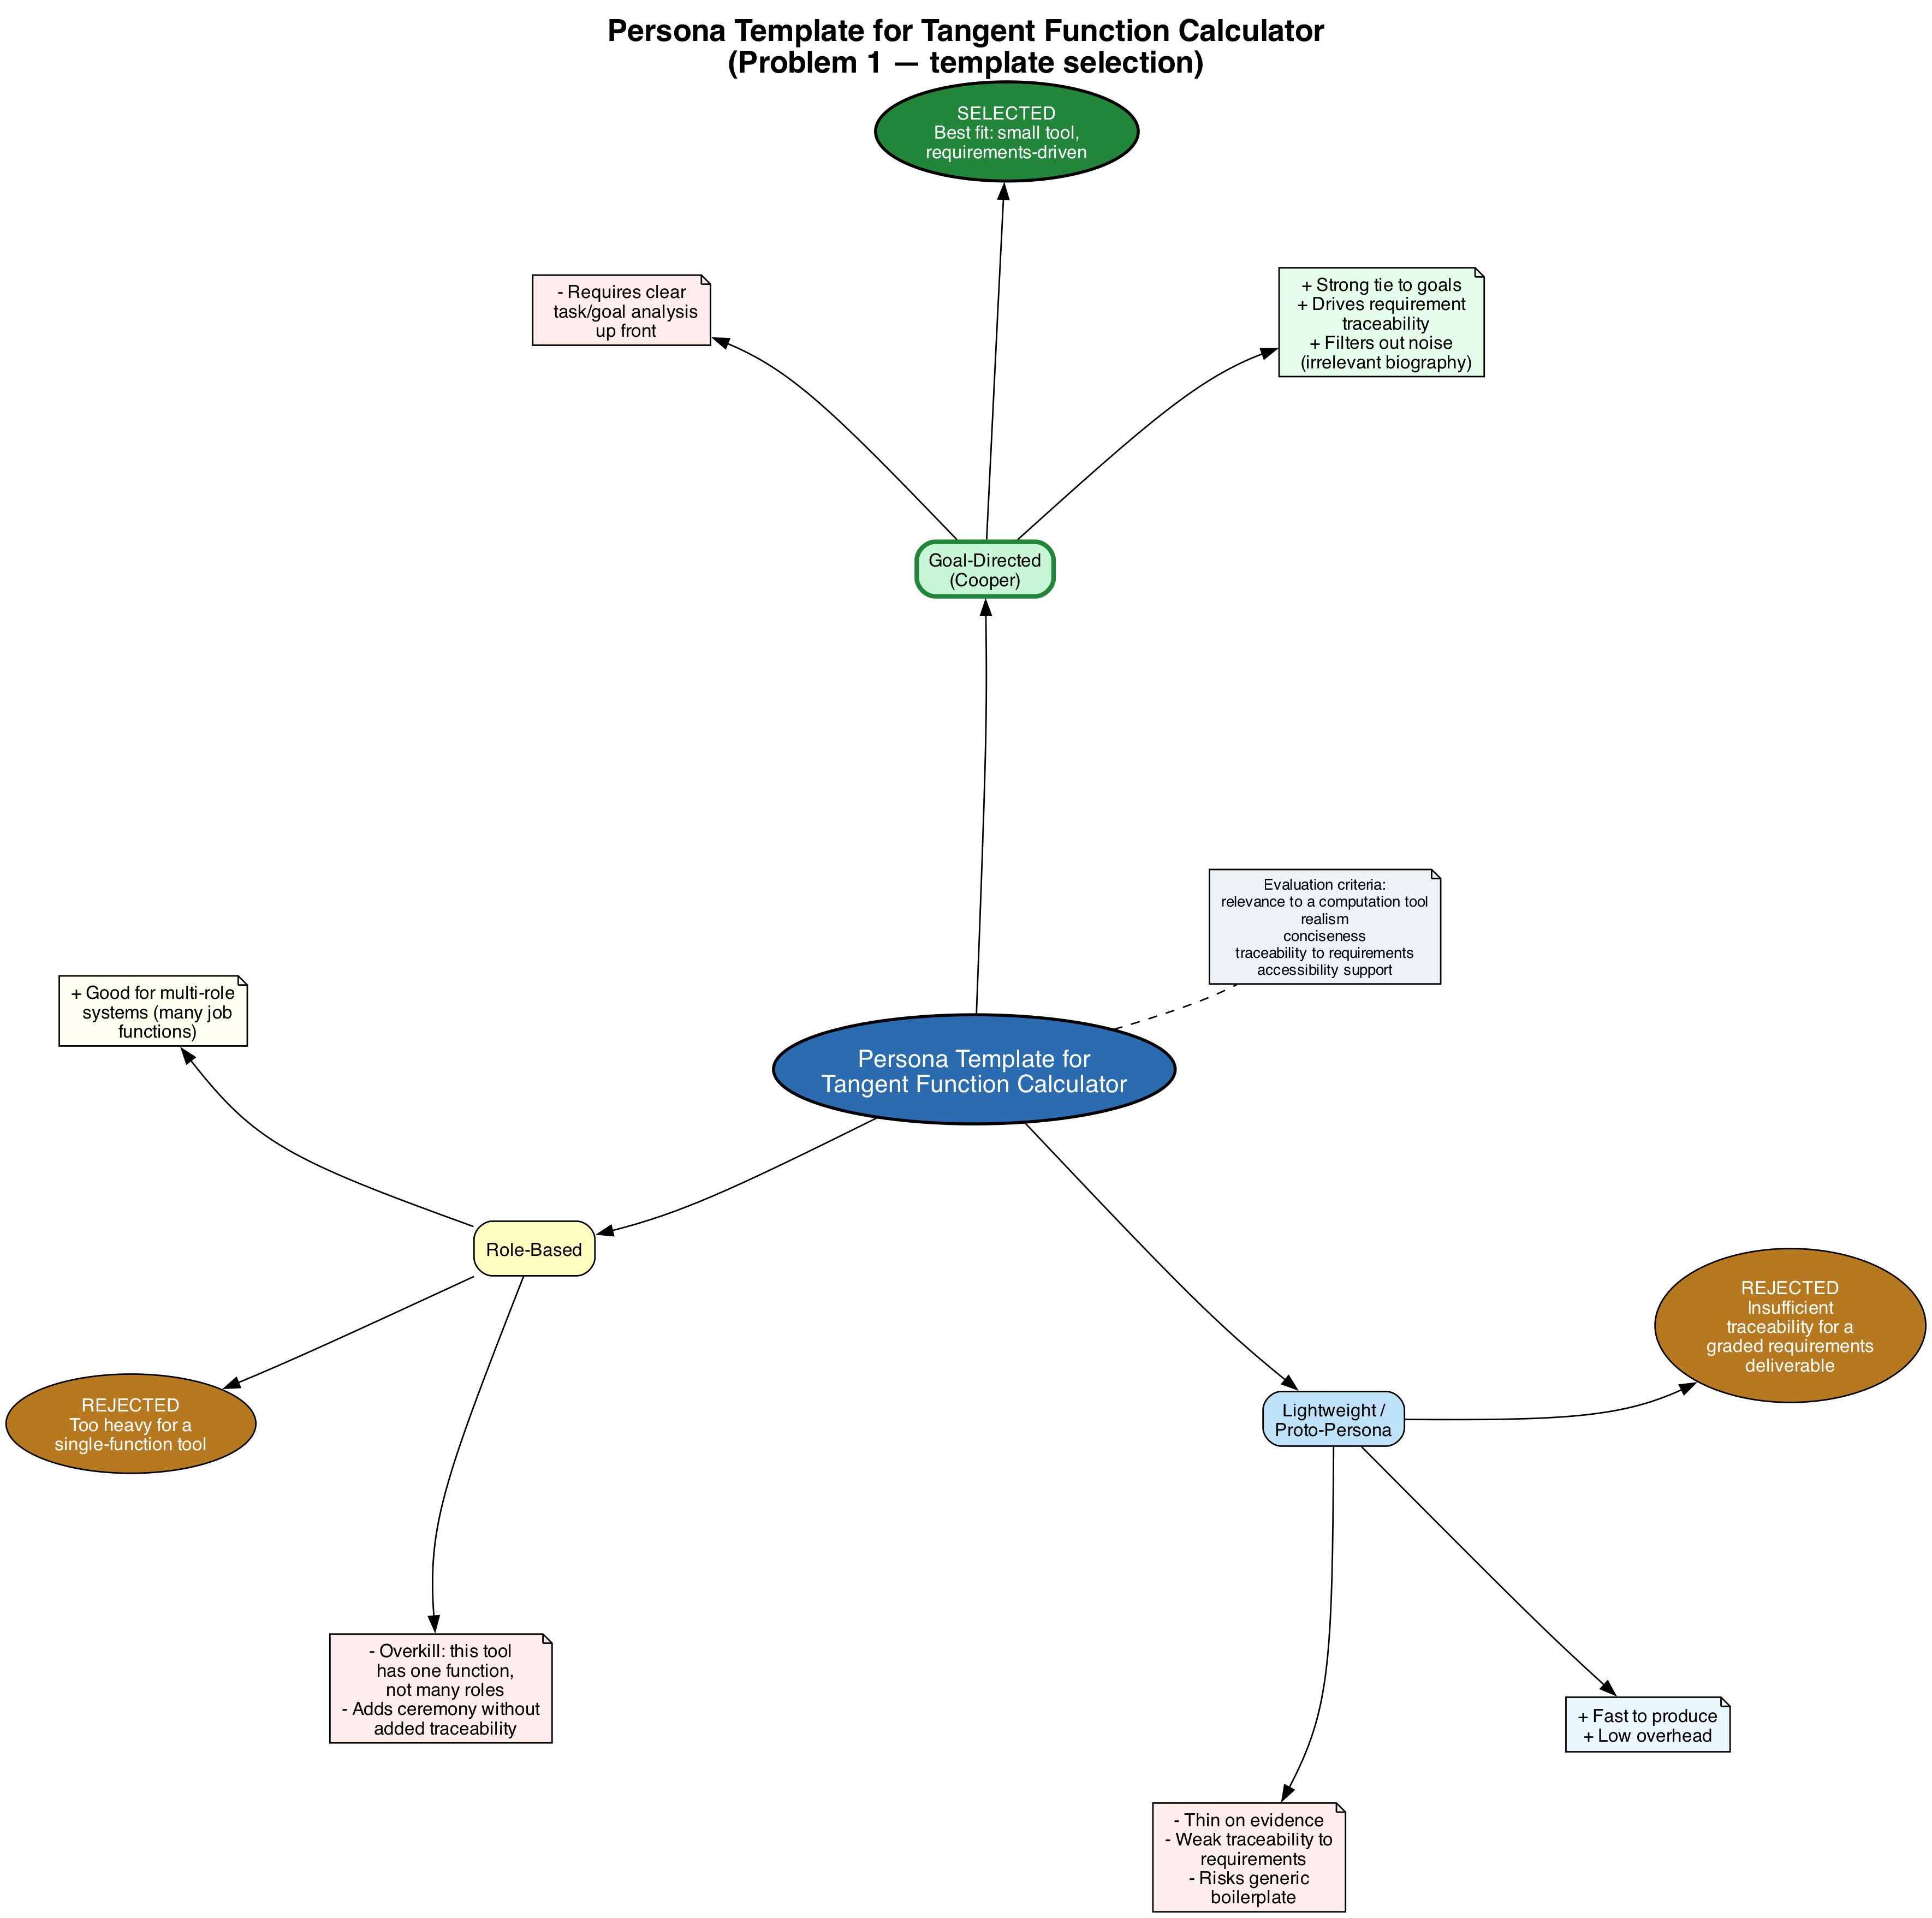
\includegraphics[width=0.92\textwidth]{../../docs/mindmaps/persona_template_mindmap.png}
  \caption{Persona-template selection mind map. Goal-directed template selected; role-based and lightweight/proto-persona rejected as too heavy or too thin on traceability, respectively.}
  \label{fig:persona-mindmap}
\end{figure}

\subsection{Persona card: Maya Chen}

\begin{longtable}{L{3.3cm}L{11.5cm}}
\toprule
\textbf{Field} & \textbf{Value} \\
\midrule
\endhead
Name & Maya Chen \\
Role / job title & M.A.Sc. student, Mechanical Engineering; part-time research assistant in an undergraduate optics teaching lab \\
Experience level & Comfortable with algebra, trigonometry, and basic scripting; not a professional software developer \\
Goals & Get a trustworthy $\tan(x)$ value quickly during a lab session without opening a full CAS; avoid a silently wrong answer from a radians/degrees mix-up \\
Working environment & Shared teaching lab and personal laptop; occasionally a bare lab machine over a slow connection; prefers a lightweight terminal tool over a full IDE or CAS \\
Tangent-specific needs & (1) Clear statement of the expected angle unit; (2) confidence that inputs near $90^\circ / \pi/2$ won't silently return a nonsensical huge number; (3) a documented precision to judge lab-report suitability; (4) a way to sanity-check a familiar special value; (5) clear, non-cryptic error messages \\
Pain points & Radians/degrees confusion; distrust of results near an asymptote; limited patience for raw tracebacks; needing quick answers without a full CAS \\
\bottomrule
\end{longtable}

\textbf{Usage scenario:} Maya is checking a refraction angle from her lab manual, given in degrees. She converts it to radians herself, enters it into the calculator (which first reminds her the input must be in radians and states the valid domain), and receives a result with documented precision. Out of curiosity she also tries an angle very close to $\pi/2$ and is relieved to see a clear "near an undefined point" message instead of a meaningless huge number.

\textbf{Evidence vs.\ synthesis vs.\ assumption:} the tangent function's mathematical properties cited above are drawn from Step 1 research notes, not invented. Maya's specific role is a plausible, illustrative composite (not a real interviewed person) of "an engineering, physics, or surveying student or lab/research assistant," per the task description. Full details, including the persona-to-requirement traceability table (7 traced needs, exceeding the $\ge 5$ gate), are in \texttt{docs/persona\_card.md}.

\section{Problem 2 --- Requirements (ISO/IEC/IEEE 29148)}

\subsection{GAI tool and prompt}
\textbf{Tool:} Claude Code (Sonnet 5). \textbf{Prompt type:} Generative + transformational (persona needs $\rightarrow$ verifiable requirements) with review. The finalized Problem 1 persona was pasted into the prompt's placeholder (full prompt in Appendix~\ref{sec:gai-log}).

\subsection{Requirements baseline v0.1}

Requirements use a single statement style ("The system shall \ldots") with IDs grouped by category: \texttt{FR} (functional), \texttt{VAL} (input validation/domain), \texttt{ACC} (accuracy/numerical), \texttt{USE} (usability), \texttt{REL} (reliability), \texttt{ERR} (error handling), \texttt{DOC} (documentation). Priorities follow Must/Should/Could.

\begin{longtable}{L{1.3cm}L{6.7cm}L{4.3cm}L{1cm}L{1.9cm}}
\toprule
\textbf{ID} & \textbf{Statement} & \textbf{Rationale (persona trace)} & \textbf{Pri.} & \textbf{Verification} \\
\midrule
\endhead
FR-01 & Accept a real-valued angle $x$ entered as text. & No CAS available. & Must & Test \\
FR-02 & State that $x$ is interpreted in radians before requesting input. & Radians/degrees confusion. & Must & Demo \\
FR-03 & Compute $\tan(x)=\sin(x)/\cos(x)$ for any $x$ accepted under VAL-01--04. & Core purpose. & Must & Test \\
FR-04 & Display the computed result as text. & Quick trustworthy result. & Must & Demo \\
FR-05 & Allow a new $x$ without restarting. & Repeated use in one session. & Should & Test \\
FR-06 & Allow exit via an explicit command. & Basic CLI usability. & Must & Demo \\
VAL-01 & Reject non-numeric input; re-prompt with a message. & No cryptic crash on typos. & Must & Test \\
VAL-02 & Reject empty input; re-prompt with a message. & Same as VAL-01. & Must & Test \\
VAL-03 & Reject $|x|$ exceeding a documented max ($10^4$ rad). & Argument-reduction error grows with $|x|$. & Must & Test \\
VAL-04 & Detect $x$ within a documented tolerance of a pole and treat as invalid. & Fear of silent huge numbers near $90^\circ$. & Must & Test \\
ACC-01 & Relative error $\le 10^{-9}$ vs.\ reference values (outside pole band, within range). & Documented precision for lab-report use. & Must & Test \\
ACC-02 & Display result to a fixed, documented number of significant figures (10). & Same as ACC-01. & Should & Inspection \\
USE-01 & State valid domain and angle unit before requesting $x$. & Radians/pole confusion. & Must & Demo \\
USE-02 & Provide a textual (CLI) interface, no GUI required. & Bare lab machine. & Must & Demo \\
REL-01 & Return control without an unhandled crash, for any input. & No cryptic crash. & Must & Test \\
REL-02 & Run from a terminal, no IDE dependency. & Shared/bare lab machine. & Must & Demo \\
ERR-01 & On rejection, name the specific violated condition. & Helpful, non-generic errors. & Must & Test \\
ERR-02 & Never propagate an unhandled Python exception for expected invalid/near-pole cases. & Same as ERR-01. & Must & Test \\
DOC-01 & Document angle unit, supported range, pole tolerance, and displayed precision. & Trust for lab-report use. & Should & Inspection \\
\bottomrule
\end{longtable}

\textbf{Assumptions (kept separate from requirements):} angle unit is radians (no degrees mode in this baseline); the pole tolerance itself is an implementation-time constant fixed in Problem 4/DOC-01; supported range is $|x|\le 10^4$ rad; no requirement prescribes an algorithm, library, or language; "numeric" input means anything Python's standard float parsing accepts.

\subsection{Quality review findings}

\begin{longtable}{L{1.6cm}L{3.3cm}L{5.3cm}L{5cm}}
\toprule
\textbf{ID (draft)} & \textbf{Characteristic at risk} & \textbf{Issue} & \textbf{Fix (adopted)} \\
\midrule
\endhead
ACC-01 & Verifiable / Unambiguous & "compute tan(x) quickly and accurately" -- unquantified. & Quantified relative-error bound vs.\ a named reference. \\
FR-03 & Feasible / no implementation prescription & Draft named "Taylor series" inside a Problem-2 requirement. & Rewritten to state only \emph{what} is computed, not \emph{how}. \\
VAL-03/04 & Singular & Draft bundled range-check and pole-check in one statement. & Split into two independently verifiable requirements. \\
\bottomrule
\end{longtable}

No requirement was found to violate necessary, complete, or consistent. A dedicated \texttt{PERF} (response-time) requirement was considered and deliberately deferred (Could-priority, not part of the persona's stated pain points). Frozen as \textbf{Requirements Baseline v0.1}; later changes (D2/Problem~7) will be recorded as a new version per constraint C-06.

\section{Problem 3 --- Two Algorithms in Pseudocode}

\subsection{GAI tool and prompt}
\textbf{Tool:} Claude Code (Sonnet 5). \textbf{Prompt type:} Generative + comparative. Relevant Problem 2 requirement IDs (ACC-01, VAL-03, VAL-04, REL-01) were pasted into the prompt's placeholder (full prompt in Appendix~\ref{sec:gai-log}).

\subsection{Algorithm A --- range reduction + Maclaurin series}

Traces to ACC-01, VAL-03, VAL-04, REL-01. Constants: \texttt{PI} (finite-precision $\pi$), \texttt{X\_MAX} (VAL-03), \texttt{EPSILON} (pole tolerance, VAL-04), \texttt{TOL} (series tolerance), \texttt{N\_MAX} (max terms).

\begin{lstlisting}[style=pseudo,caption={Algorithm A: TAN-BY-SERIES},label={lst:algoA}]
TAN-BY-SERIES(x, PI, X_MAX, EPSILON, TOL, N_MAX)
 1  if |x| > X_MAX
 2      signal RANGE-ERROR                    // VAL-03
 3      return
 4  s <- 1
 5  if x < 0                                   // odd symmetry: tan(-x) = -tan(x)
 6      x <- -x
 7      s <- -s
 8  k <- ROUND(x / (PI / 2))                   // nearest multiple of pi/2
 9  r <- x - k * (PI / 2)                      // r in [-pi/4, pi/4]
10  j <- k mod 2
11  sinR <- MACLAURIN-SIN(r, TOL, N_MAX)
12  cosR <- MACLAURIN-COS(r, TOL, N_MAX)
13  if j = 0
14      num <- sinR ; den <- cosR
15  else                                       // tan(r + pi/2) = -cos(r)/sin(r)
16      num <- -cosR ; den <- sinR
17  if |den| < EPSILON
18      signal POLE-ERROR                      // VAL-04
19      return
20  return s * (num / den)

MACLAURIN-SIN(r, TOL, N_MAX)
 1  term <- r ; sum <- r ; n <- 1
 2  while |term| >= TOL and n <= N_MAX          // max-work safeguard
 3      term <- term * (-(r * r)) / ((2n) * (2n+1))
 4      sum <- sum + term ; n <- n + 1
 5  return sum

MACLAURIN-COS(r, TOL, N_MAX)
 1  term <- 1 ; sum <- 1 ; n <- 1
 2  while |term| >= TOL and n <= N_MAX          // max-work safeguard
 3      term <- term * (-(r * r)) / ((2n-1) * (2n))
 4      sum <- sum + term ; n <- n + 1
 5  return sum
\end{lstlisting}

\textbf{Termination:} bounded unconditionally by \texttt{N\_MAX} regardless of tolerance. \textbf{Complexity:} $O(\texttt{N\_MAX})$ per call, a fixed constant ($\sim$10--15 terms for $10^{-12}$ relative error). \textbf{Weaknesses:} argument-reduction error grows with $|x|$ (finite-precision \texttt{PI}); catastrophic cancellation in the reduction subtraction for large $x$; precision loss just outside the \texttt{EPSILON} guard band.

\textbf{Worked trace, $\tan(\pi/4)=1$:} $k=\mathrm{ROUND}(0.5)=0$ (round-half-to-even), $r=\pi/4$, $j=0$. The sine series gives $\mathrm{sum} \approx 0.7854, 0.7046, 0.70714, 0.710270, \ldots \to 0.70710678$ after a few terms; the cosine series converges symmetrically to the same value. Result: $s \cdot (\mathrm{num}/\mathrm{den}) = 1 \cdot (0.70710678/0.70710678) = 1$, matching the reference value.

\subsection{Algorithm B --- CORDIC (circular mode, rotation mode)}

Same requirement trace as Algorithm A, reached by a structurally different method. Reuses the identical sign-and-quadrant reduction. Constants additionally include a precomputed table $A[i] = \arctan(2^{-i})$, computed once offline (not via a built-in \texttt{arctan} inside the algorithm).

\begin{lstlisting}[style=pseudo,caption={Algorithm B: TAN-BY-CORDIC},label={lst:algoB}]
TAN-BY-CORDIC(x, PI, X_MAX, EPSILON, A[0..N_MAX-1], N_MAX)
 1  if |x| > X_MAX
 2      signal RANGE-ERROR                    // VAL-03
 3      return
 4  s <- 1
 5  if x < 0
 6      x <- -x ; s <- -s
 7  k <- ROUND(x / (PI / 2))
 8  r <- x - k * (PI / 2)                      // r in [-pi/4, pi/4]
 9  j <- k mod 2
10  (cosR, sinR) <- CORDIC-ROTATE(r, A, N_MAX)
11  if j = 0
12      num <- sinR ; den <- cosR
13  else                                       // tan(r + pi/2) = -cos(r)/sin(r)
14      num <- -cosR ; den <- sinR
15  if |den| < EPSILON
16      signal POLE-ERROR                      // VAL-04
17      return
18  return s * (num / den)

CORDIC-ROTATE(r, A[0..N_MAX-1], N_MAX)
 1  vx <- 1 ; vy <- 0 ; z <- r
 2  for i <- 0 to N_MAX - 1                    // fixed count: max-work safeguard
 3      if z >= 0 : d <- +1  else d <- -1
 4      vx_next <- vx - d * vy * 2^(-i)         // shift, not divide
 5      vy_next <- vy + d * vx * 2^(-i)
 6      z <- z - d * A[i]
 7      vx <- vx_next ; vy <- vy_next
 8  K <- GAIN-CONSTANT(N_MAX)                  // product of cos(A[i]), precomputed
 9  return (vx / K, vy / K)                    // (cos(r), sin(r))
\end{lstlisting}

\textbf{Optimization note:} since $\tan(r) = (K\sin r)/(K\cos r) = vy/vx$, the gain constant $K$ cancels exactly when only $\tan$ is needed. \textbf{Termination:} exactly \texttt{N\_MAX} iterations, unconditional. \textbf{Complexity:} $O(\texttt{N\_MAX})$ shift-add operations only (no multiply/divide in the loop). \textbf{Weaknesses:} linear convergence (~1 bit/iteration, needing $\sim$40 iterations for $10^{-12}$ precision, versus 10--15 series terms for Algorithm A); finite table precision caps ultimate accuracy; shares Algorithm A's range-reduction risks.

\textbf{Worked trace, $\tan(\pi/4)=1$:} starting from $(vx,vy,z)=(1,0,0.785398)$, the rotation sequence gives $vy/vx = 1.0, 3.0, 1.571, 1.209, 1.066, 1.0013, 0.9705, 0.9858, \ldots$ after iterations $0$--$7$, then $0.99741$ at $i{=}9$, $0.999997$ at $i{=}19$, and $1.000000000000$ at $i{=}39$ -- confirming both correctness and the linear-convergence weakness noted above (all values independently computed, not via a built-in \texttt{tan}).

\subsection{How A and B differ}

\begin{longtable}{L{3.2cm}L{5.6cm}L{5.6cm}}
\toprule
\textbf{Dimension} & \textbf{Algorithm A (Maclaurin)} & \textbf{Algorithm B (CORDIC)} \\
\midrule
\endhead
Core arithmetic & Multiplication and division every term & Only addition/subtraction/shift \\
Convergence & Super-linear (factorial growth), $\sim$10--15 terms & Linear ($\sim$1 bit/iter), $\sim$40 iterations \\
Termination & Tolerance-or-cap \texttt{while} loop & Fixed-count \texttt{for} loop \\
Precomputed constants & \texttt{PI} only & $\arctan(2^{-i})$ table (+ optional gain $K$) \\
D2 from-scratch fit & Needs from-scratch multiply/divide & Strong fit -- shift/add only in hot loop \\
Explainability & High -- "the Taylor series from calculus" & Moderate -- needs a rotation mental model \\
\bottomrule
\end{longtable}

The two algorithms differ in core technique, arithmetic primitives, convergence class, and termination mechanism -- not superficial variants of one idea.

\section{Problem 4 --- Algorithm Selection + Python CLI}

\subsection{GAI tool and prompt}
\textbf{Tool:} Claude Code (Sonnet 5). \textbf{Prompt type:} Decision-support (mind map) + generative (Python). Both Problem 3 algorithms were pasted into the prompt's placeholder (full prompt in Appendix~\ref{sec:gai-log}).

\subsection{Selection mind map}

\begin{figure}[htbp]
  \centering
  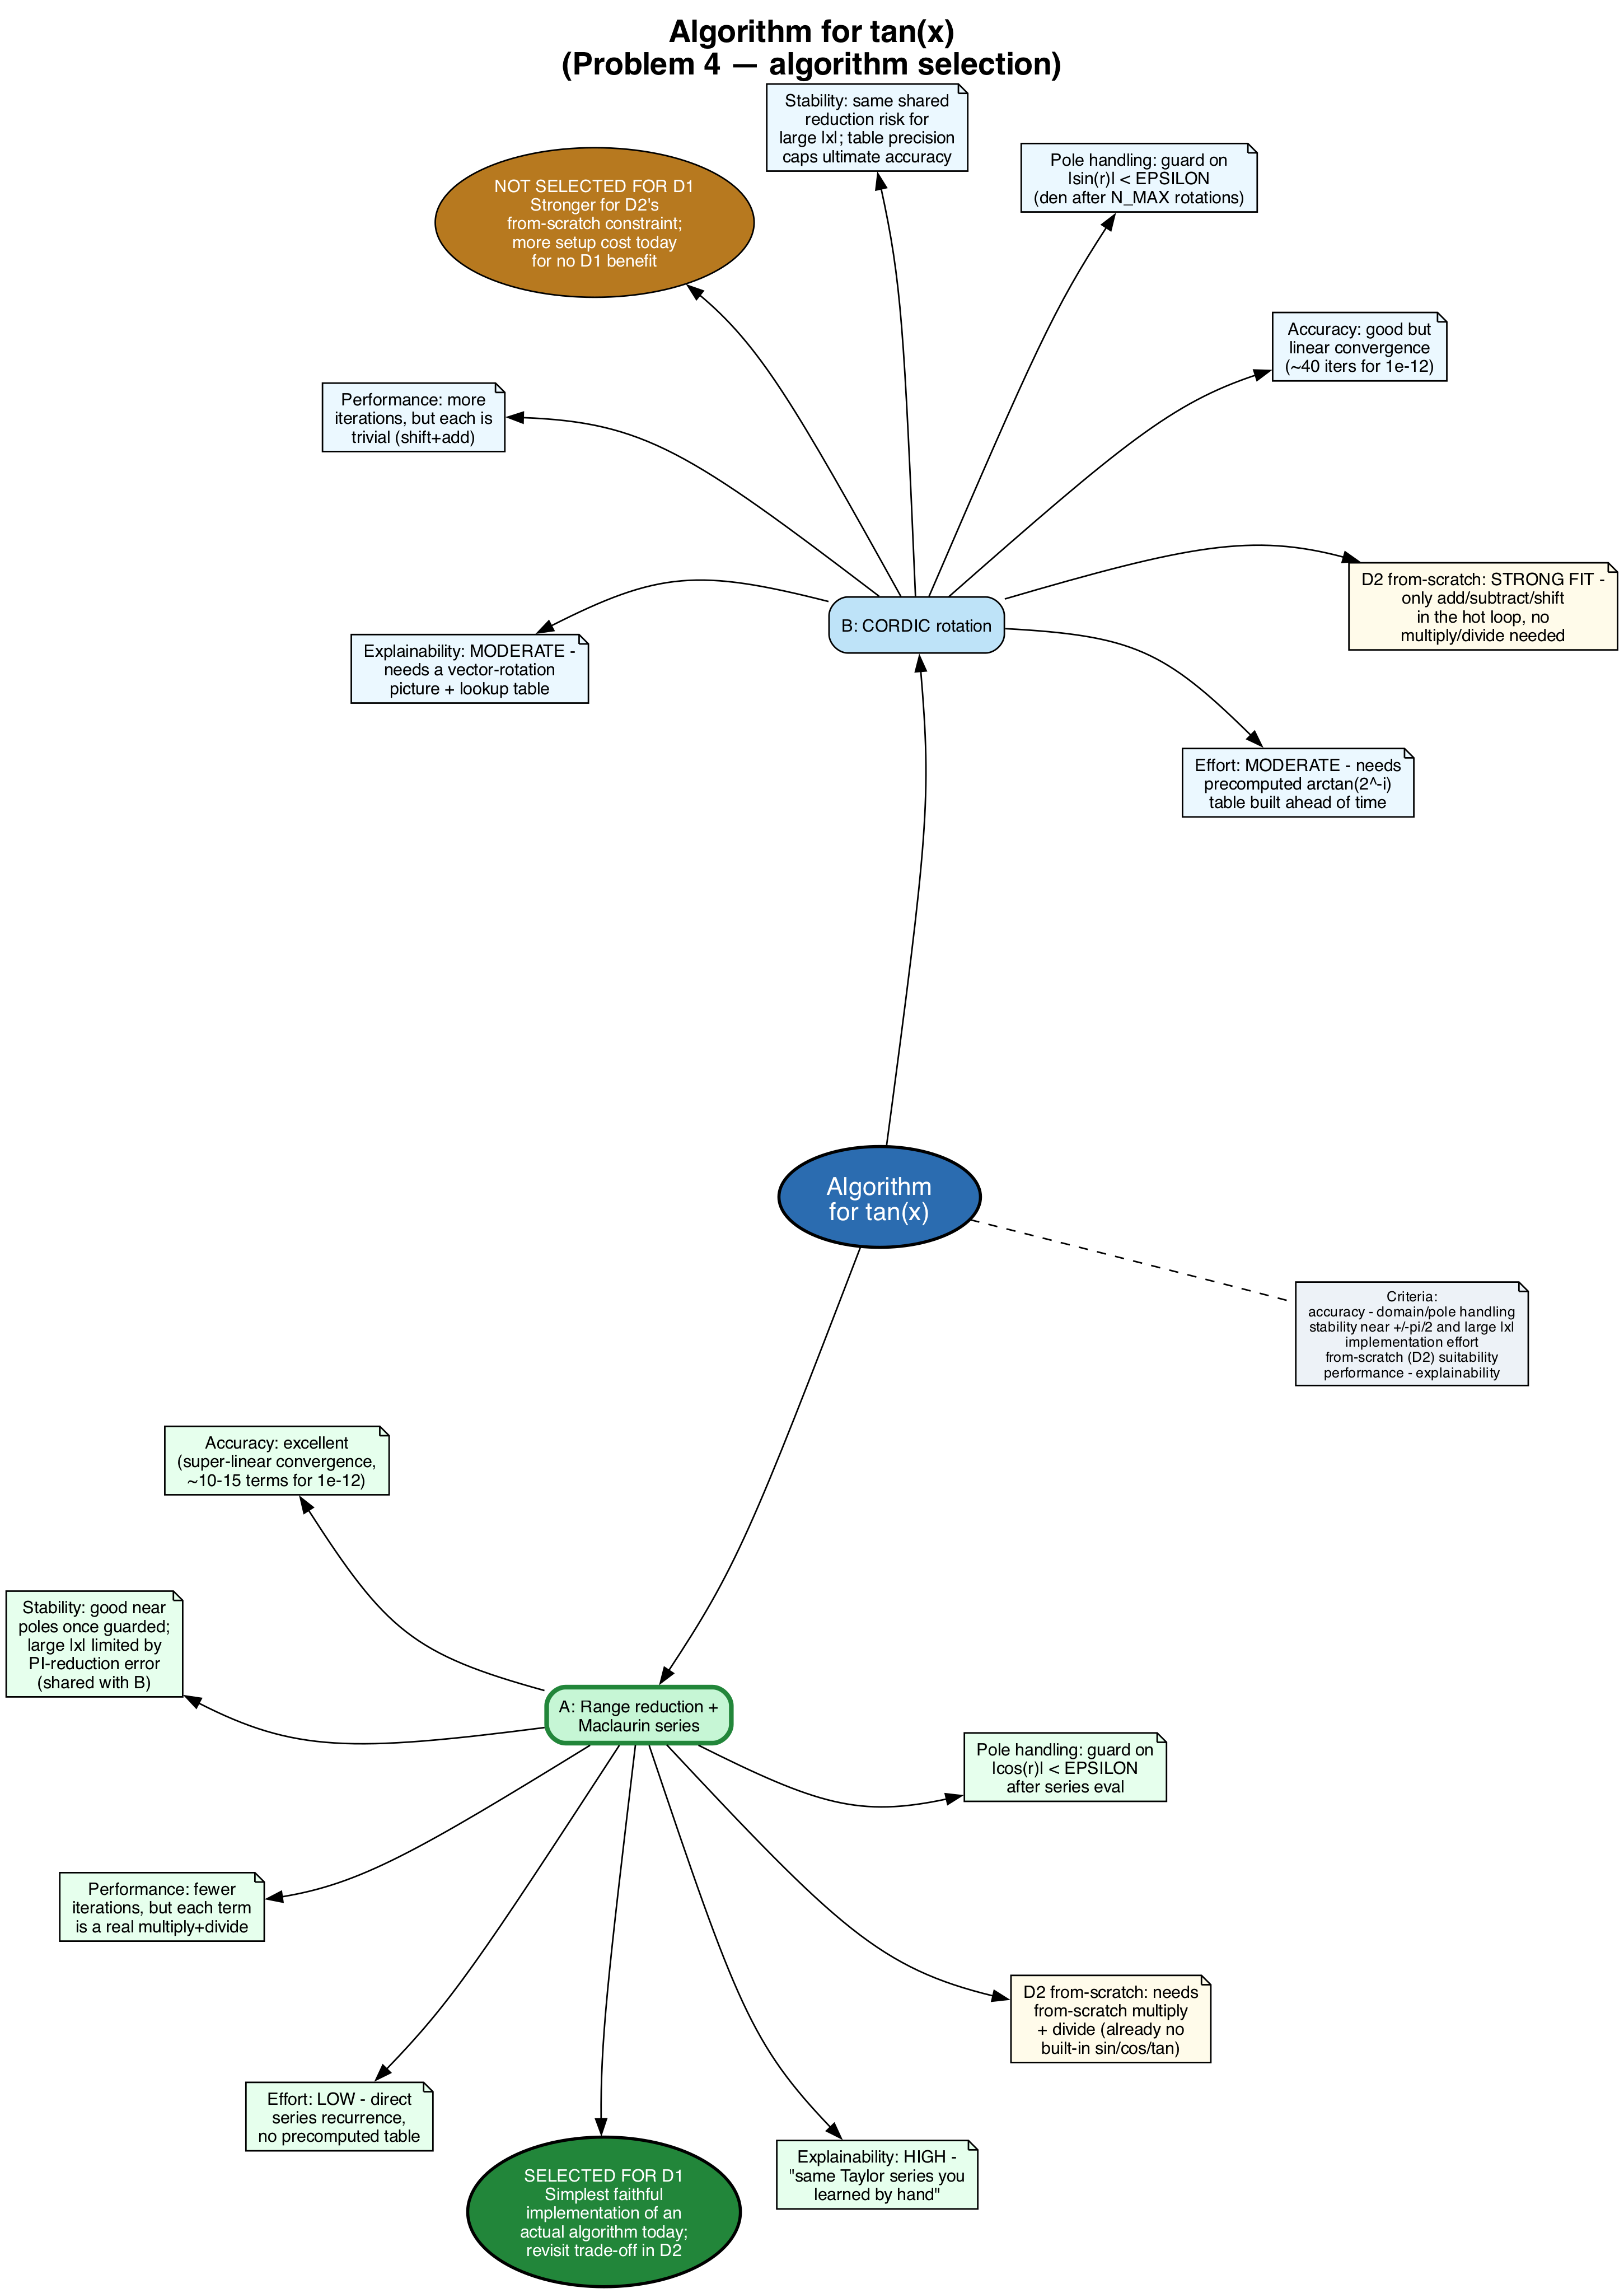
\includegraphics[width=0.72\textwidth,height=0.82\textheight,keepaspectratio]{../../docs/mindmaps/algorithm_selection_mindmap.png}
  \caption{Algorithm-selection mind map. Algorithm A selected for the D1 prototype on implementation effort and explainability; Algorithm B noted as the stronger candidate for D2's from-scratch constraint.}
  \label{fig:algo-mindmap}
\end{figure}

\textbf{Selection: Algorithm A.} It is the simplest way to faithfully implement an actual algorithm today, is most explainable to the persona, and has the lowest implementation effort. Algorithm B's multiplication-free hot loop is a D2 concern, not a D1 one, so it does not outweigh A's simplicity here; the decision will be revisited in Deliverable 2.

\subsection{Python CLI implementation}

\texttt{src/cli.py} separates a pure \textbf{compute layer} (\texttt{maclaurin\_sin}, \texttt{maclaurin\_cos}, \texttt{tan\_by\_series} -- implementing Algorithm A exactly) from an \textbf{I/O layer} (\texttt{run\_cli}, \texttt{parse\_x}, \texttt{format\_result}). Two custom exceptions, \texttt{OutOfRangeError} (VAL-03) and \texttt{NearPoleError} (VAL-04), are raised by the compute layer and caught individually in the I/O loop, each producing a distinct helpful message (ERR-01) -- never an unhandled traceback (ERR-02, REL-01). The angle unit and valid-domain hint are stated in the banner before the first prompt (USE-01, FR-02); results display to 10 significant figures (ACC-02, DOC-01).

\begin{lstlisting}[style=code,caption={Core compute function (excerpt), src/cli.py},label={lst:cli-core}]
def tan_by_series(x):
    if abs(x) > X_MAX:
        raise OutOfRangeError(...)
    sign = 1.0
    if x < 0:
        x = -x
        sign = -1.0                     # tan(-x) = -tan(x)
    k = round(x / (PI / 2))
    r = x - k * (PI / 2)                 # r in [-pi/4, pi/4]
    quadrant_flip = (k % 2) == 1
    sin_r = maclaurin_sin(r)
    cos_r = maclaurin_cos(r)
    if quadrant_flip:
        numerator, denominator = -cos_r, sin_r
    else:
        numerator, denominator = sin_r, cos_r
    if abs(denominator) < POLE_EPSILON:
        raise NearPoleError(...)
    return sign * (numerator / denominator)
\end{lstlisting}

\textbf{D2 from-scratch note:} this implementation already computes \texttt{sin}/\texttt{cos} itself via the Maclaurin series; neither \texttt{math.sin} nor \texttt{math.cos} appears in the compute path. The one remaining standard-library dependency is \texttt{PI = math.pi}, which D2 must replace with an independently derived constant.

\subsection{Sample runs}

\begin{longtable}{L{3.4cm}L{3.2cm}L{7.8cm}}
\toprule
\textbf{Case} & \textbf{Input} & \textbf{Output} \\
\midrule
\endhead
Valid (special value) & $x=\pi/4$ & \texttt{tan(0.7853981634) = 1} \\
Negative (odd symmetry) & $x=-\pi/4$ & \texttt{tan(-0.7853981634) = -1} \\
Boundary/near-pole & $x=\pi/2-10^{-9}$ & \texttt{Cannot compute tan(x): x is at or within tolerance of a pole ...} \\
Invalid (non-numeric) & \texttt{"abc"} & \texttt{Invalid input: 'abc' is not a valid real number. ...} \\
Missing input & \texttt{""} & \texttt{Invalid input: No input received. ...} \\
Large argument (supported) & $x=1000$ & \texttt{tan(1000) = 1.470324156} \\
Large argument (out of range) & $x=10^{10}$ & \texttt{Input out of range: |x| = 1e+10 exceeds the supported range ...} \\
\bottomrule
\end{longtable}

Figure~\ref{fig:screenshots} shows two representative rendered terminal transcripts (all four, plus raw \texttt{.txt} transcripts, are in \texttt{docs/screenshots/}).

\begin{figure}[htbp]
  \centering
  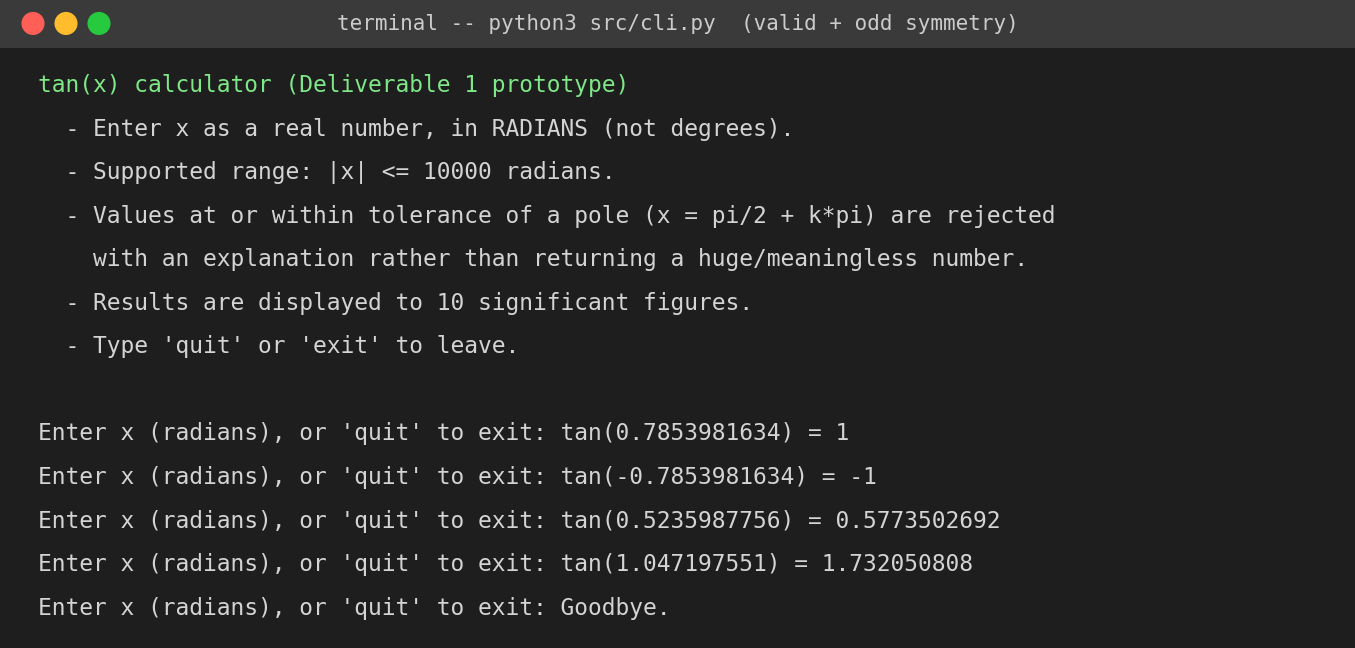
\includegraphics[width=0.85\textwidth]{../../docs/screenshots/run1_valid_and_odd_symmetry.png}\\[0.3cm]
  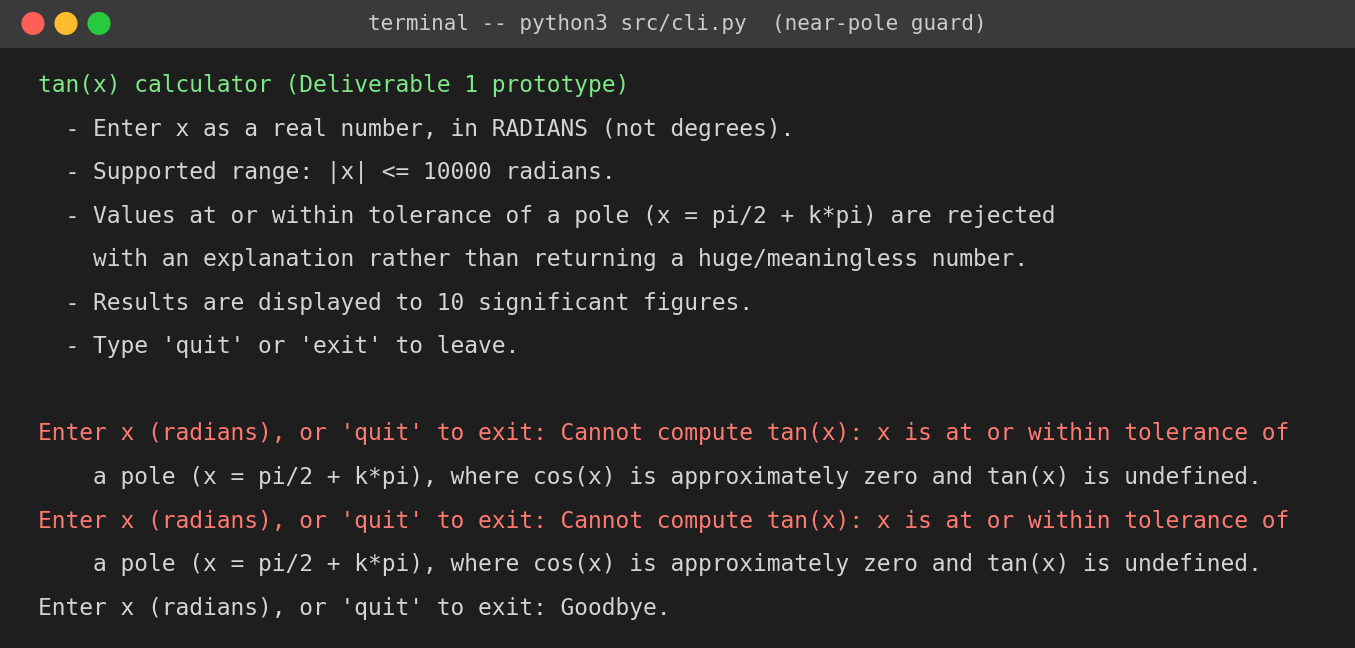
\includegraphics[width=0.85\textwidth]{../../docs/screenshots/run3_near_pole.png}
  \caption{Sample CLI runs: valid values with odd symmetry (top), and near-pole rejection on both sides of a pole (bottom).}
  \label{fig:screenshots}
\end{figure}

\section{Verification (Step 6)}

Table~\ref{tab:verify} ties requirement IDs to demo cases and results, cross-checked against \texttt{docs/research\_notes.md} and an independent \texttt{math.tan} computation (never the CLI's own output used as its own reference).

\begin{longtable}{L{3.6cm}L{3.4cm}L{3.4cm}L{3.4cm}}
\caption{Verification matrix (abridged; full matrix in \texttt{docs/verification\_matrix.md}).}
\label{tab:verify} \\
\toprule
\textbf{Requirement ID(s)} & \textbf{Demo case} & \textbf{Reference} & \textbf{Verdict} \\
\midrule
\endfirsthead
\multicolumn{4}{l}{\textit{Table~\ref{tab:verify} continued}} \\
\toprule
\textbf{Requirement ID(s)} & \textbf{Demo case} & \textbf{Reference} & \textbf{Verdict} \\
\midrule
\endhead
FR-01,03,04,ACC-01 & $x=\pi/4$ & $\tan(\pi/4)=1$ & Pass \\
ACC-01, odd symmetry & $x=-\pi/4$ & $\tan(-\pi/4)=-1$ & Pass \\
VAL-04, ERR-01/02, REL-01 & $x=\pi/2-10^{-9}$ & undefined (pole) & Pass (rejected) \\
VAL-04, ERR-01/02, REL-01 & $x=-\pi/2$ & undefined (pole) & Pass (rejected) \\
VAL-01, ERR-01, REL-01 & \texttt{"abc"} & n/a & Pass (rejected) \\
VAL-02, ERR-01, REL-01 & \texttt{""} & n/a & Pass (rejected) \\
ACC-01, VAL-03 & $x=1000$ & $1.470324156$ & Pass \\
VAL-03, ERR-01, REL-01 & $x=10^{10}$ & n/a (out of range) & Pass (rejected) \\
FR-05/06, USE-01/02, REL-02 & multi-input session + quit/EOF & clean exit both ways & Pass \\
\bottomrule
\end{longtable}

\textbf{Known limitations (honest disclosure):} large-argument accuracy degrades gradually below the $|x|\le 10^4$ cutoff (not yet quantified precisely, deferred to D2/D3 with a higher-precision reference); the pole tolerance ($10^{-6}$) and $X\_MAX$ ($10^4$) are provisional constants pending professor confirmation; no performance/timing requirement was verified (deliberately deferred); the reference values themselves rely on Python's finite-precision \texttt{math.tan}, adequate for this deliverable's $10^{-9}$--$10^{-10}$ target but not an arbitrary-precision oracle.

\section{Decision Rationale}
\label{sec:decisions}

Key decisions from the running decision log (\texttt{docs/decisions/decision\_log.md}):

\begin{itemize}
  \item \textbf{D-01/D-02/D-03 (provisional, pending professor confirmation):} angle unit is radians; near-pole inputs are rejected via an \texttt{EPSILON}-tolerance guard rather than computed; supported range is $|x|\le 10^4$ rad.
  \item \textbf{D-04:} this deliverable's scope covers Problems 1--4 (persona, requirements, two algorithms, selection+CLI).
  \item \textbf{D-05:} Algorithm B (Problem 3) is CORDIC rather than the Lentz continued-fraction alternative, since CORDIC is structurally more different from Algorithm A and generalizes better to the D2 from-scratch constraint.
\end{itemize}

\section{Implementation Summary}

\texttt{src/cli.py} implements Algorithm A end-to-end: range reduction modulo $\pi/2$ with sign/quadrant tracking, Maclaurin series for $\sin$/$\cos$ with a tolerance-or-cap stopping rule, a pole guard, and a textual I/O loop satisfying every Must-priority requirement in the Section 2 baseline. All sample runs in Section 4.4 and the verification matrix in Section 5 were produced by this exact source file with no modification.

\appendix
\section{GAI Prompt Log (summary)}
\label{sec:gai-log}

Per constraint C-03, the exact CASTROFF prompts (Task/Restrictions/Output~Format/Audience) for all four problems are in \texttt{SOEN\_6011\_F2\_D1\_Prompts.md}, and the full evaluation log (GAI tool, output summary, critical evaluation of accepted/rejected/corrected content, verification method, attribution) is in \texttt{docs/prompts/gai\_prompt\_log.md}. All four problems used the same tool: Claude Code (Claude, Anthropic, Sonnet 5 model), accessed 2026-07-15. In every case, at least one part of the raw output was rejected or corrected before being adopted (documented per problem in that log) -- for example, an early Problem 2 draft used unquantified terms ("fast and accurate") and was rewritten as a quantified relative-error bound, and an early Problem 4 draft called \texttt{math.sin}/\texttt{math.cos} directly and was corrected to call the from-scratch series functions instead, consistent with actually implementing the selected algorithm rather than wrapping a library call.

\begin{thebibliography}{9}
\bibitem{cooper2007} A. Cooper, R. Reimann, and D. Cronin, \emph{About Face 3: The Essentials of Interaction Design}. Wiley, 2007.
\bibitem{pruitt2006} J. Pruitt and T. Adlin, \emph{The Persona Lifecycle: Keeping People in Mind Throughout Product Design}. Morgan Kaufmann, 2006.
\bibitem{iso29148} ISO/IEC/IEEE, \emph{ISO/IEC/IEEE 29148:2018 -- Systems and Software Engineering -- Life Cycle Processes -- Requirements Engineering}, 2018.
\bibitem{volder1959} J. E. Volder, ``The CORDIC Trigonometric Computing Technique,'' \emph{IRE Transactions on Electronic Computers}, vol. EC-8, no. 3, pp. 330--334, 1959.
\bibitem{muller2016} J.-M. Muller et al., \emph{Handbook of Floating-Point Arithmetic}, 2nd ed. Birkh\"auser, 2016.
\bibitem{cormen2009} T. H. Cormen, C. E. Leiserson, R. L. Rivest, and C. Stein, \emph{Introduction to Algorithms}, 3rd ed. MIT Press, 2009.
\bibitem{abramowitz1964} M. Abramowitz and I. A. Stegun, \emph{Handbook of Mathematical Functions with Formulas, Graphs, and Mathematical Tables}. National Bureau of Standards, 1964.
\bibitem{nist_dlmf} NIST, \emph{NIST Digital Library of Mathematical Functions}, \url{https://dlmf.nist.gov/}, 2026.
\end{thebibliography}

\end{document}
